% 0.5 page

\subsection{Bithoven}
\label{project-description-bithoven}
Bithoven is a music information service, specializing in classical music. A
common problem with existing music streaming services is their lack of support
for metadata usually desired for classical music. Things like composer,
conductor, soloist(s), content group, etc. are often nowhere to be found.
Enter: Bithoven.

Users of Bithoven will be able to sign into their account in order to search
pieces using the formerly mentioned metadata. That way, if the user listens to
a piece and enjoys a specific part of it, they will be able to quickly find out
who was responsible for it and can explore their other pieces. The users will
also be able to create playlists, containing any pieces they like.

\subsection{UML Model}
\label{project-description-uml}
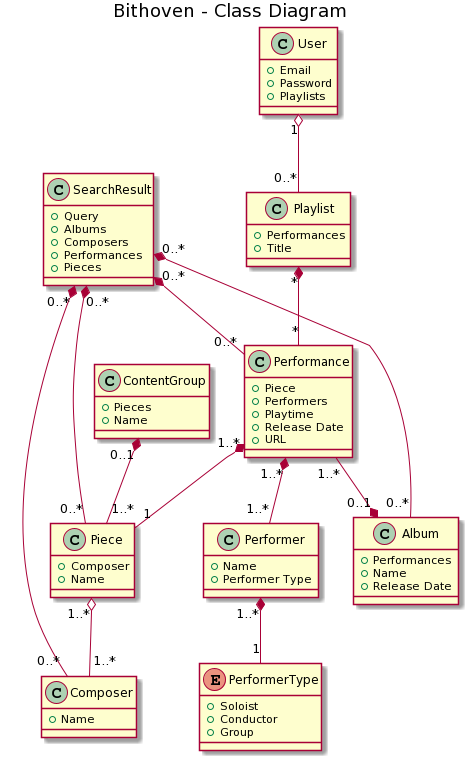
\includegraphics[scale=0.5]{uml.png}

\subsection{Requirements}
\label{project-description-req}

\begin{enumerate}
    \item User can sign up for an account with an e-mail account and password.
    \item User can sign into their account by providing corresponding e-mail
        account and password.
    \item User can view all owned playlists.
    \item User can view all performances in a certain playlist.
    \item User can create new playlists.
    \item User can delete playlists.
    \item User can modify name of playlist.
    \item User can add performances to playlists.
    \item User can delete performances from playlists.
    \item User can search for albums, composers, content groups, pieces,
        performers, performances through free text.
    \item System provides search results from a query grouped into the provided
        category.
    \item System can provide metadata for user to explore.
    \item System can list all pieces and content groups by composer.
    \item System can list all performances of a certain piece or content group.
    \item System can list all performances by performer/album.
    \item System can list all pieces in a content group.
    \item System can list information about a specific performance.
    \item A piece has the following properties: 1 composer, composition date, a
        title.
    \item A piece may specify a content group, and in that case an order.
    \item A performance has the following properties: 1 piece, at least 1
        performer, 0 or 1 album, release date, playtime, and a URL to the
        recording.
    \item A performance in an album must specify its track number.
    \item A performer must have at least one of the following roles in a
        performance: soloist, group, conductor.
    \item A performer must have a name. 
    \item An album must have a title and release date.
    \item A composer must have a name.
\end{enumerate}
